\section{Ustalenia terminologiczne}\label{sub:terms}
\begin{definicja}[Graf skierowany (DG)]\label{def:DG}
Powiedzmy, że:
\begin{enumerate}
\item \(V\neq\emptyset\) jest zbiorem
\item \( E \subseteq V \times V \)
\end{enumerate}
Grafem skierowanym \(G\) nazwiemy dwójkę \((V, E)\).
\end{definicja}

\begin{definicja}[Acykliczny graf skierowany (DAG)]\label{def:dag}
Acyklicznym grafem skierowanym nazywamy graf skierowany nie zawierający cykli.
\end{definicja}

\begin{definicja}[Domknięcie przechodnie grafu]\label{def:domk_przechodnie_grafu}
Niech \(G=(V,A)\) będzie grafem skierowanym. Graf skierowany \(G^+=(V,A^{+})\) nazywamy \textbf{domknięciem przechodnim} grafu \(G\), gdy \(A^{+}\) jest zbiorem wszystkich takich par \((a,b)\) wierzchołków zbioru \(V\), że w grafie \(G\) istnieje droga z \(a\) do \(b\).
\end{definicja}

\begin{definicja}[Zbiór przechodni]\label{def:transitive_set}
Zbiór \(A\) nazywamy \textbf{przechodnim}, wtedy i tylko wtedy, gdy
\(\forall{x}\left(x\in A \land y\in x\implies y\in A\right)\).  
\end{definicja}

\begin{definicja}[Domknięcie przechodnie zbioru]\label{def:transitive_closure_set}
Domknięciem przechodnim zbioru \(X\) nazywamy najmniejszy w sensie inkluzji zbiór przechodni, który zawiera \(X\).
\end{definicja}

\begin{definicja}[Graf zależności]\label{def:depend_graph}
Niech dane będą zbiór \(S\neq\emptyset\), relacja przechodnia \(R\subseteq S\times S\). \textbf{Grafem zależności} nazywamy graf \(G=(S,T)\) i \(T\subseteq R\), gdzie \(R\) jest przechodnim domknięciem \(T\).
\end{definicja}


\begin{definicja}[Ścieżka]\label{def:sciezka}
\textbf{Ścieżką} łączącą \(v_0\) z \(v_n\) o długości \(n\) nazywamy ciąg wierzchołków \((v_0, v_1, \dots, v_n)\) taki, że dla każdego \(k\in \{0, 1, \dots, n-1\}\) istnieje krawędź z \(v_k\) do \(v_{k+1}\).
\end{definicja}

\begin{definicja}[Droga]\label{def:droga}
\textbf{Drogą} w grafie \(G\) nazywamy ścieżkę, której wierzchołki są różne.
\end{definicja}

\begin{definicja}[Długość drogi]\label{def:dlugosc_drogi}
\textbf{Długością} drogi w grafie \(G\) nazywamy liczbę krawędzi, które zawiera droga.
\end{definicja}
\begin{definicja}[Cykl]\label{def:cykl_w_grafie}
Drogę zamkniętą długości co najmniej 1 z ciągiem wierzchołków \(x_1 x_2\dots x_n x_1\) nazywamy \textbf{cyklem}, jeśli wszystkie wierzchołki\\ \(x_1, x_2\dots x_n\) są różne.
\end{definicja}

\begin{definicja}[Stopień wierzchołka]\label{def:stopien_node}
\textbf{Stopień \(d_{G}(v)\) wierzchołka} \(v\) definiujemy jako liczbę incydentnych z \(v\) krawędzi. Każdemu wierzchołkowi \(v\) grafu skierowanego \(G\) możemy przypisać stopień wyjściowy (ang. \emph{indegree}) \(d_{G}^{+}(v)\) i stopień wejściowy (ang. \emph{outdegree}) \(d_{G}^{-}(v)\):
\begin{align*}
 d_{G}^{+}(v) = \#\{w|(v,w)\in E\}\\ 
 d_{G}^{-}(v) = \#\{w|(w,v)\in E\}
\end{align*}
\end{definicja}

\begin{definicja}[Macierz]\label{def:matrix}
Niech \(\mathbb{K}\) będzie ciałem. Macierzą o \(m\) wierszach i \(n\) kolumnach i wartościach w \(\mathbb{K}\) (krótko: macierzą \(m\times n\)) nazywamy każde odwzorowanie \(A:\{1,\dots, m\}\times \{1, \dots, n\}\xrightarrow{} \mathbb{K}, (i,j)\longmapsto A_{ij}\)
\end{definicja}

\newpage

\section{Klasyfikacja algorytmów}\label{sub:algorithms}
\begin{definicja}[Algorytm]\label{def:algorytm}
Zbiór jednoznacznie określonych reguł lub zadań obliczeniowych prowadzących w skończonej ilości kroków do rozwiązania pewnego problemu \cite{IEEE}.
\end{definicja}


Określone w ten sposób zadania obliczeniowe są z reguły względem siebie niezależne. Pewne z zadań mogą być wykonywane równolegle, inne muszą być wykonywane sekwencyjnie, jedno po drugim. Wobec tego algorytm może być określony częściowo równolegle, częściowo sekwencyjnie.


Podstawowymi elemetami określającymi dowolny algorytm są:
\begin{enumerate}
\item zadania do wykoniania,
\item zależności pomiędzy zadaniami polegające na określeniu czy 
dane wyjściowe któregoś z zadań nie są danymi wejściowymi dla innego zadania,
\item zbiór danych wejściowych wymaganych przez algorytm,
\item zbiór danych wyjściowych otrzymywanych po wykonania algorytmu.
\end{enumerate}

%Na podstawie niezależności zadań obliczeniowych algorytmy możemy %podzielić na pięć klas \cite{APC2011}:
%\begin{enumerate}
%\item Algorytmy szeregowe
%\item Algorytmy równoległe
%\item Algorytmy szeregowo--równoległe (SPA, Serial--Parallel %Algorithms)
%\item Algorytmy nieszeregowo--równoległe (NSPA, Nonserial--%Parallel Algorithms)
%\item Algorytmy regularno-iteracyjne (RIA, Regular--Iterative %Algorithms)
%\end{enumerate}

\begin{definicja}[Algorytm sekwencyjny]\label{def:algorytm_sekwencyjny}
\textbf{Algorytm sekwencyjny} (rys.  \ref{fig:sequential}) jest ciągiem dokładnie sprecyzowanych zadań obliczeniowych \(T_i,\, i\in\mathbb{N}\) rozwiązujących dany problem, tj. wyznaczających dane wyjściowe na podstawie danych wejściowych. Zakłada się, że w algorytmie sekwencyjnym zadania wykonywane są przez jeden procesor.

\end{definicja}

\begin{figure}[h]
\centering
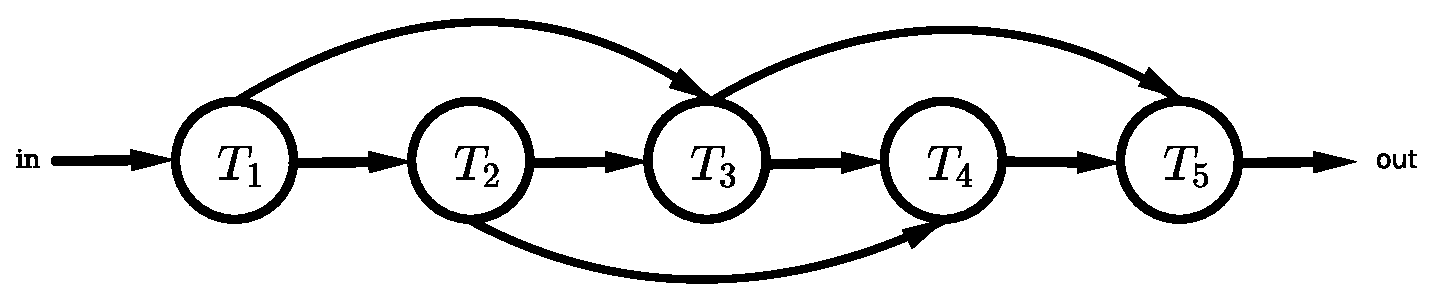
\includegraphics[width=14cm]{images/Rys2.eps}
\caption{Algorytm sekwencyjny}
\label{fig:sequential}
\end{figure}

W celu rozwiązania problemu za pomocą większej liczby procesorów należy go zdekomponować na podproblemy, które mogą być rozwiązane równolegle. Każdy z podproblemów rozwiązywany jest przez odrębny algorytm będący składową algorytmu równoległego.


\begin{definicja}[Równoległość]\label{def:rownoleglosc}
\textbf{Równoległość} w odniesieniu do oprogramowania jest to symultaniczny transfer, występowanie albo przetwarzanie poszczególnych części pewnej całości, takich jak bity składające się na znak albo znaki pewnego słowa, używając osobnych urządzeń dla ich różnych części \cite{IEEE}.
\end{definicja}


\begin{definicja}[Algorytm równoległy]\label{def:algorytm_rownolegly}
\textbf{Algorytmem równoległym} (rys. \ref{fig:parallel}) nazywamy każdy algorytm, w którym spośród określonych w nim zadań \(T_1\), \(T_2\), \(\dots\), \(T_n\) co najmniej dwa zadania \(T_i\), \(T_j\), \(i\neq j\) dzięki ich wzajemnej niezależności, mogą być wykonane równocześnie \cite{APC2011}.\\
\end{definicja}

\begin{figure}[h]
\centering
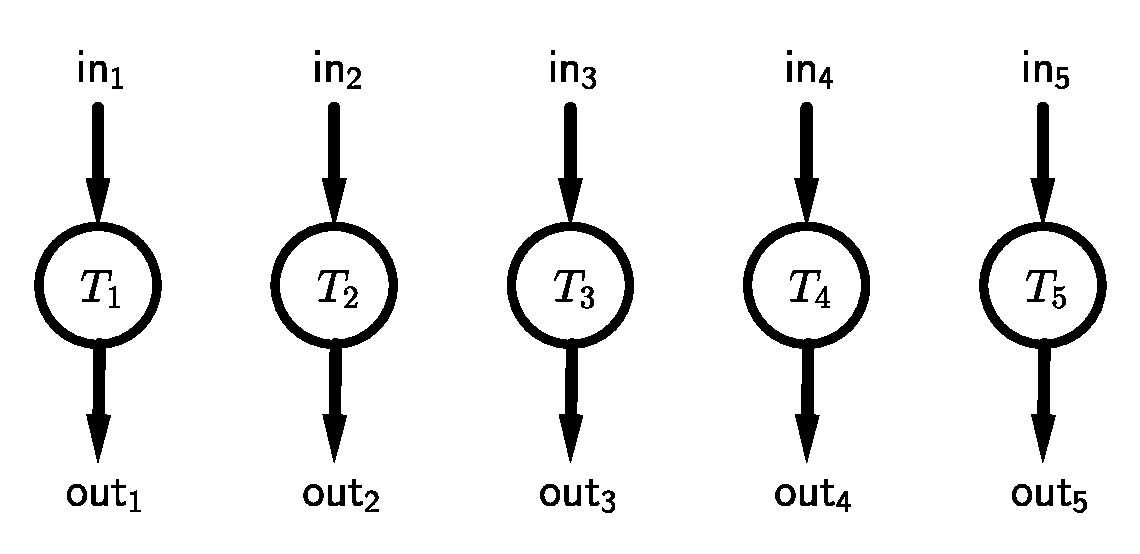
\includegraphics[width=10cm]{images/Rys1.eps}
\caption{Algorytm równoległy}
\label{fig:parallel}
\end{figure}



%
%\begin{definicja}[Algorytmy szeregowo--równoległe]
%
%\end{definicja}
%
%\begin{definicja}[Algorytmy nieszeregowo--równoległe]
%\end{definicja}
%
%\begin{definicja}[Algorytmy regularno--iteracyjne]
%Algorytmy tej klasy reprezentowane za pomocą grafów zależności wyrażają pewien pewien ustalny schemat postępowania.
%\end{definicja}

\section{Architektury równoległe}\label{sub:architectures}
\begin{definicja}[Architektura równoległa]\label{def:arch_rownolegla}
\textbf{Architektura równoległa} jest to architektura wieloprocesorowa, na której można wykonywać przetwarzanie równoległe \cite{IEEE}.
\end{definicja}

Algorytmy równoległe i architektury równoległe są ze sobą blisko spokrewnione. Równoległość może być zaimplementowana na wielu poziomach używając technik sprzętowych i programowych.
\begin{enumerate}
\item{Równoległość na poziomie danych (ang. \emph{Data-level parallelism}), gdzie pracujemy na wielu bitach danych lub na wielu danych jednocześnie.}
\item{Równoległość na poziomie instrukcji (ang. \emph{Instruction-level parallelism}, ILP), gdzie jednocześnie procesor może wykonać więcej niż jedną instrukcję.}
\item{Równoległość na poziomie wątków (ang. \emph{Thread-level parallelism}, TLP). Wątek jest częścią programu, która współdzieli zasoby procesora z innymi wątkami. W TLP wiele programowych wątków jest uruchamianych jednocześnie na jednym bądź wielu procesorach.}
\item{Równoległość na poziomie procesów (ang. \emph{Process-level parallelism}). Proces to program, który jest uruchomiany na komputerze. Rezerwuje on własne zasoby komputera, takie jak przestrzeń pamięciową i rejestry.\cite{APC2011}}
\end{enumerate}

\begin{przyklad}
Prostym przykładem algorytmu równoległego jest serwer siecowy, który każde zapytanie przychodzące przetwarza niezależnie od innych zapytań. Innym przykładem są wielozadaniowe systemy operacyjne radzące sobie z jednoczesną obsługą kilku uruchomionych programów.
\end{przyklad}

\subsubsection{Klasyfikacja Flynna}
Architektury komputerowe można podzielić na klasy ze względu na liczbę równolegle wykonywanych instrukcji oraz dostępnych strumieni danych. Klasyfikację taką (rys. \ref{fig:flynn}) zaproponował Michael J. Flynn w 1966 roku i przyjęła ona swoją nazwę od jego nazwiska (rys. \ref{fig:flynn}).

\begin{figure}
\centering
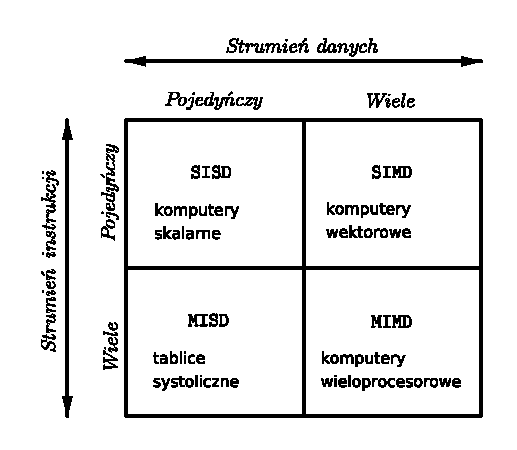
\includegraphics[width=24em]{images/flynn.eps}
\caption{Klasyfikacja Flynna}
\label{fig:flynn}
\end{figure}

\paragraph{SISD.}
Klasa SISD (ang. \emph{Single Instruction, Single Data}) odnosi się do komputerów wykonujących pojedyńczy strumieniem instrukcji i przetwarzających pojedyńczy strumień danych. Są to komputery całkowicie sekwencyjne, które nie wykonują żadnych obliczeń równoległych.
\paragraph{SIMD.}
Klasa SIMD (ang. \emph{Single Instruction, Multiple Data}) odnosi się do komputerów obsługujących pojedyńczy strumień instrukcji i przetwarzających wiele strumieni danych. Na różnych zbiorach danych wykownywane są te same operacje. Jako przykład takiej architektury warto wymienić przede wszystkim wczesne komputery macierzowe (nazywane niekiedy wektorowymi) ze wspólną pamięcią i macierzą jednostek przetwarzających nadzorowanych przez jednostkę sterującą, takie jak komputer ILLIAC IV wykorzystywany przez NASA w latach '70.
\paragraph{MISD.}
Klasa MISD (ang. \emph{Multiple Instruction, Single Data}) 
odnosie się do komputerów wykonujących jednocześnie wiele instrukcji przetwarzających jeden współny strumien danych. Przykładem takiej architektury jest tablica systoliczna\footnote{Nazwa pochodzi od skurczu mięśni serca przez analogię ,,pompowania'' danych do jednostek przetwarzających na wzór krwi w naczyniach krwionośnych.}. Tablica systoliczna jest to układ prostych jednostek przetwarzających połączonych w sieć z sąsiadującymi jednostkami, które synchronicznie wykonują pewne elementarne operacje obliczeniowe.
\paragraph{MIMD.}
Klasa MIMD  (ang. \emph{Multiple Instruction, Multiple Data})
odnosi się do komputerów równolegle wykonujących wiele instrukcji z których każda przetwarza własne strumienie danych. Do tej kategorii zaliczają się multiprocesory\footnote{Komputery z wieloma jednostkami centralnymi przyłączonymi do pamięci współdzielonej (ang. \emph{shared memory}.)} (większość współczesnych komputerów PC) i multikomputery\footnote{Wiele komputerów połączonych siecią, każdy z własną przestrzenią adresową.}. 


Większość obecnie używanych komputerów równoległych to klastry o architekturze mieszanej. Klaster jest układem niezależnych jednostek obliczeniowych (węzły) połączonych szybką siecią komunikacyjną.\cite{OstrowskiByszewski}. 

\section{Reprezentacja algorytmów}\label{sub:representation}
Wiele obliczeń możemy repezentować za pomocą acyklicznych grafów skierowanych. Każde wejście jest oznaczane przez węzeł bez dochodzących do niego łuków. Operacje oznaczamy przez węzły do których wchodzą łuki z innych węzłów oznaczających argumenty (operandy). Stopień wejściowy dowolnego węzła wynosi co najwyżej 2. Węzeł, którego stopień wyjściowy jest równy 0 oznacza wyjście. Zakładamy, że każdy węzeł przedstawia operację, która wymaga jednej jestostki czasu wykonania.\\



Za pomocą acyklicznych grafów skierowanych możemy analizować zachowanie równoległych algorytmów przy założeniu, że każdy z procesorów ma dostęp do danych obliczonych przez inny procesor bez dodatkowych narzutów. Implementacja algorytmu polega na \emph{planowaniu} wykonania każdego węzła na wybranym procesorze.
%\begin{figure}[h]
%\centering
%\includegraphics[width=34em]{Rys3.eps}
%\caption{Algorytm macierzenia macierzy przedstawiony za pomocą DAG'a}
%\label{fig:example_dag}
%\end{figure}

Powiedzmy, że dla danych \(p\) procesorów, chcemy przyporządkować każdemu węzłowi \(i\) parę \((j_i, t_i)\), gdzie \(j_i \leq p\) oznacza indeks procesora, zaś \(t_i\) jednostkę czasu, taką że zachodzą poniższe warunki:
\begin{enumerate}
\item Jeśli \(t_i=t_k\) dla pewnego \(i\neq k\), to \(j_i\neq j_k\). Oznacza to, że każdy procesor może wykonać pojedyńczą operację podczas każdej jednostki czasu.
\item Jeśli \((i, k)\) jest łukiem grafu, to \(t_k\geq t_i + 1\). Oznacza to, że operacja, którą przedstawia węzeł \(k\) powinna być zaplanowana po wykonaniu operacji przedstawionej przez węzeł \(i\).
\end{enumerate}

Przyjmuje się, że czas \(t_i\) węzła wejściowego \(i\) wynosi 0 oraz żaden procesor nie jest przyporządkowany do tego węzła.\\
\begin{definicja}[Plan]\label{def:plan}
Ciąg \(\{(j_i, t_i) | i\in N\}\) nazywamy \textbf{planem} równoległego wykonania DAG przez \(p\) procesorów, gdzie \(N\) oznacza zbiór węzłów DAG.
\end{definicja}


Dla dowolnego planu, odpowiadający mu czas wykonania (złożoność czasowa) algorytmu jest określony przez \(\max_{i\in N}t_i\). Złożoność równoległa DAG'a jest określona przez \(T_{p}(n) = \min{\{\max_{i\in N}t_i\}}\), gdzie minimum bierzemy po wszystkich planach, które używają \(p\) procesorów.


\begin{przyklad}
Niech \(\mathbf{A}\), \(\mathbf{B}\in\mathbb{R}^{n\times n}\). Rozważmy algorytm obliczający iloczyn macierzy \(AB = C\). Każdy element \(C(i, j)\) obliczamy za pomocą wyrażenia \(C(i, j)=\sum_{l=1}^{n}A(i,l)B(l,j)\). Odpowiadający temu obliczeniu DAG dla \(n=4\) przedstawia rys. \ref{fig:standard_parallel}. Mając \(n^3\) procesorów, poszczególne operacje mogą być zaplanowane poziom po poziomie, używając \(n\) procesorów do obliczenia każdego z elementów macierzy wynikowej \(C\). Stąd widać, że możemy zaplanować DAG do obliczenia o złożoności \(O(\log{n})\)
\begin{figure}[H]
\centering
\includegraphics[width=34em]{images/Rys3.eps}
\caption{Iloczyn macierzowy, algorytm w postaci grafu.}
\label{fig:standard_parallel}
\end{figure}

\end{przyklad}

\section{Ocena algorytmów}\label{sub:performance_measures}
\label{subsec:algorytmy_sekwencyjne}
\subsubsection{Złożoność czasowa algorytmów sekwencyjnych}

Ograniczenia zasobów (np. czasu i przestrzeni) wymagane przez algorytmy sekwencyjne mierzymy jako funkcję rozmiaru danych wejściowych \(T(n)\), tzw. złożoność czasową. Ograniczenia te wyrażamy asymptotycznie używając notacji:

\begin{enumerate}
\item{\(T(n) = O(f(n))\), jeśli istnieje dodatnie stałe \(c\) i \(n_0\) takie, że \(\forall{n \geq n_0}: (T(n)\leq cf(n)) \)}
\item{\(T(n) = \Omega(f(n))\), jeśli istnieje dodatnie stałe \(c\) i \(n_0\) takie, że \(\forall{n \geq n_0}: (T(n)\geq cf(n)) \)}
\item{\(T(n) = \Theta(f(n))\), jeśli \(T(n)=O(f(n))\) i \(T(n)=\Omega(f(n))\)}
\end{enumerate}
Czas działania algorytmu sekwencyjnego szacuje się przez liczbę operacji podstawowych wymaganych przez algorytm jako funkcję ilości danych wejściowych.
\subsubsection{Złożoność czasowa algorytmów równoległych}

\begin{definicja}[Pesymistyczna złożoność obliczeniowa\cite{Czech}]\label{def:pesymistyczna_zlozonosc_czasowa}
Załóżmy że algorytm równoległy \(R\) rozwiązuje problem \(P\) o rozmiarze \(n\). \textbf{Pesymityczną złożonością czasową algorytmu} \(R\) nazywamy funkcję:\\
\begin{align}
T_{p}(n) = \sup_{d\in{D_n}}{\left\{t(p,d)\right\}},
\end{align}
gdzie \(t(p,d)\) oznacza liczbę kroków obliczeniowych (operacji dominujących) wykonanych dla zestawu danych \(d\) od momentu rozpoczęcia obliczeń algorytmu \(R\) przez pierwszy procesor do chwili zakończenia obliczeń przez wszystkie procesory, \(p\) -- liczbę procesorów, \(D_n\) -- zbiór wszystkich zestawów danych wejściowych \(d\) o rozmiarze \(n\).
\end{definicja}

\newpage

\section{Teoretyczne modele obliczeń}\label{sub:computation_models}
\subsection{Model RAM}
Nim przejdziemy do omówienia modeli obliczeń równoległych zajmiemy się omówieniem modelu odpowiadającego maszynom sekwencyjnym. 


Model RAM (\emph{Random Access Machine}) odpowiada rozważaniom zawartym w \ref{subsec:algorytmy_sekwencyjne}. Zakłada on:
\begin{enumerate}
\item{Istnienie pewnego procesora wyposażonego w:
\begin{enumerate}
\item skończoną listę instrukcji, które może on realizować (tabela \ref{tab:ram_instructions}).
\item pewną liczbę rejestrów arytmetycznych procesora \(R_1, R_2, \dots, R_n\), \(n>1\) które mogą przechowywać dowolne skończone liczby w zapisie binarnym.
\item specjalny rejestr sterujący \(L\) zwany licznikiem programu.
\end{enumerate}}
\item Istnienie pamięci złożonej z potencjalnie nieskończonej liczby komórek \(M_i, \, i=1, 2, 3, \dots\) (rys. \ref{fig:neumann}) w których można przechowywać dowolną skończoną liczbę w zapisie binarnym.
\item Stały czas zapisu i odczytu wartości do/z komórki pamięci (inaczej \emph{dostęp swobodny}).

\end{enumerate}


\begin{figure}[h]
\centering
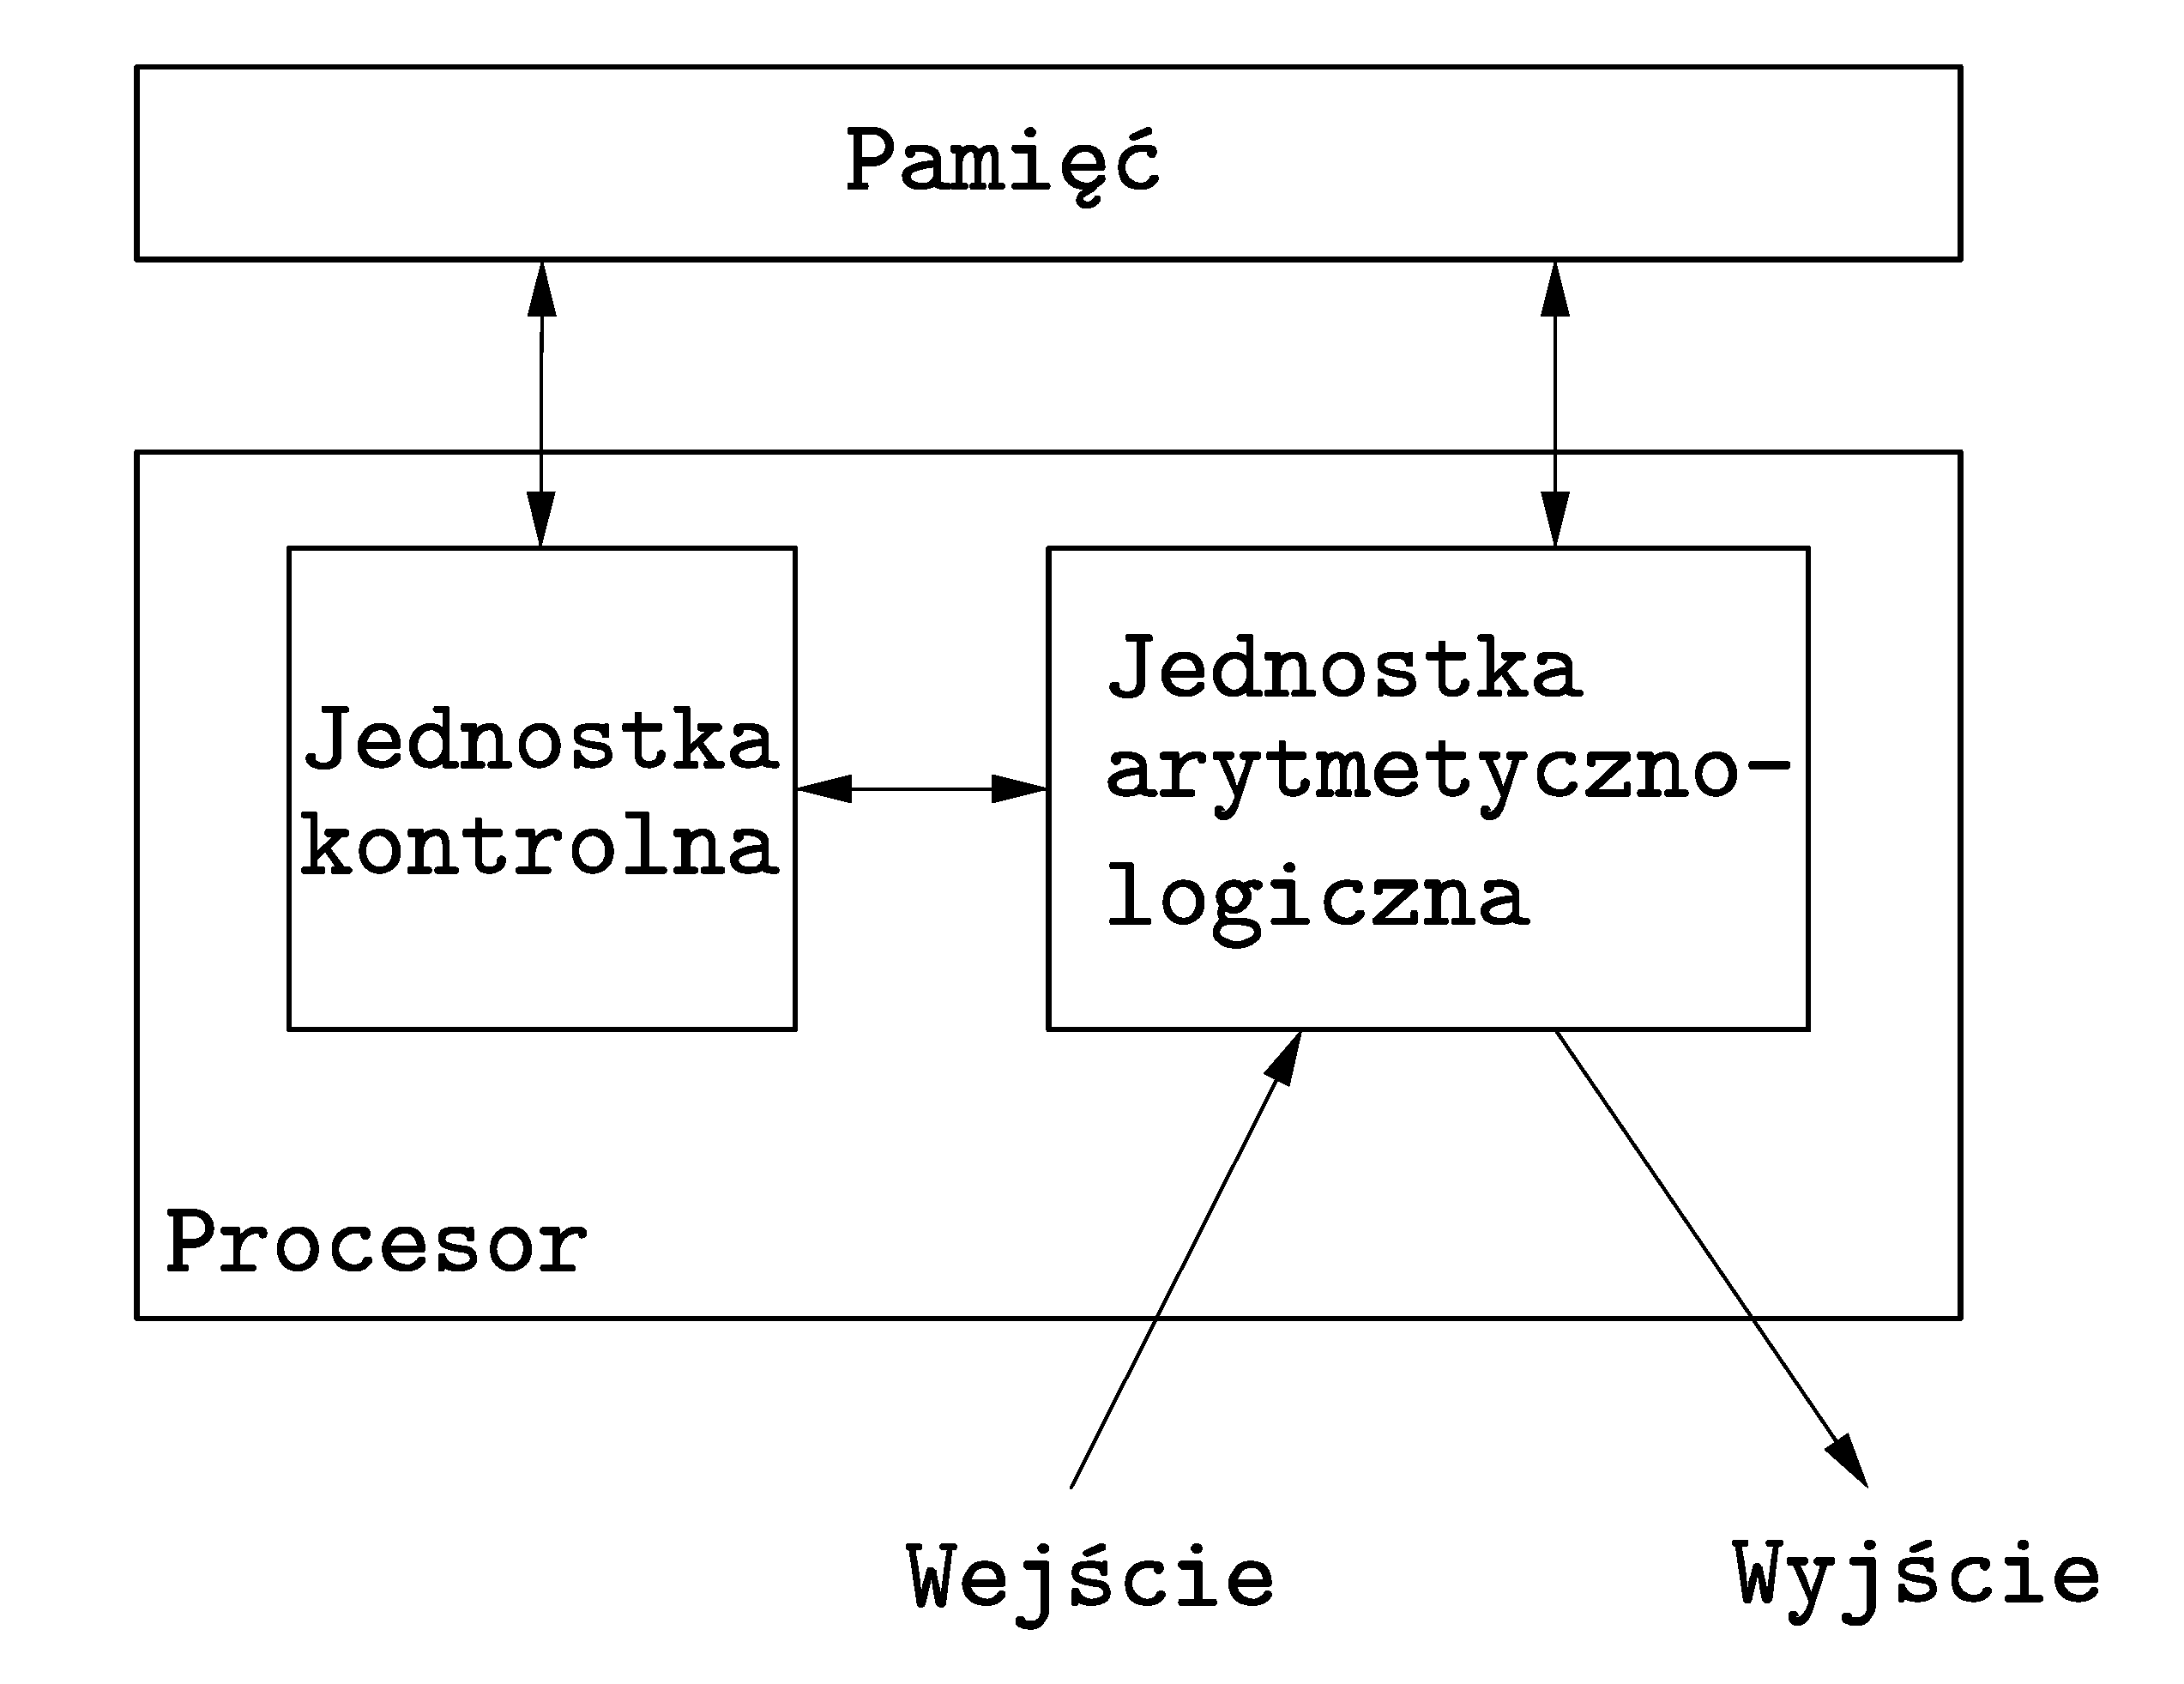
\includegraphics[width=9cm]{images/Rys_Neumann.eps}

\caption{Model obliczeń sekwencyjnych RAM – architektura Von Neumanna}
\label{fig:neumann}
\end{figure}


% \begin{figure}[h]
% \centering
% 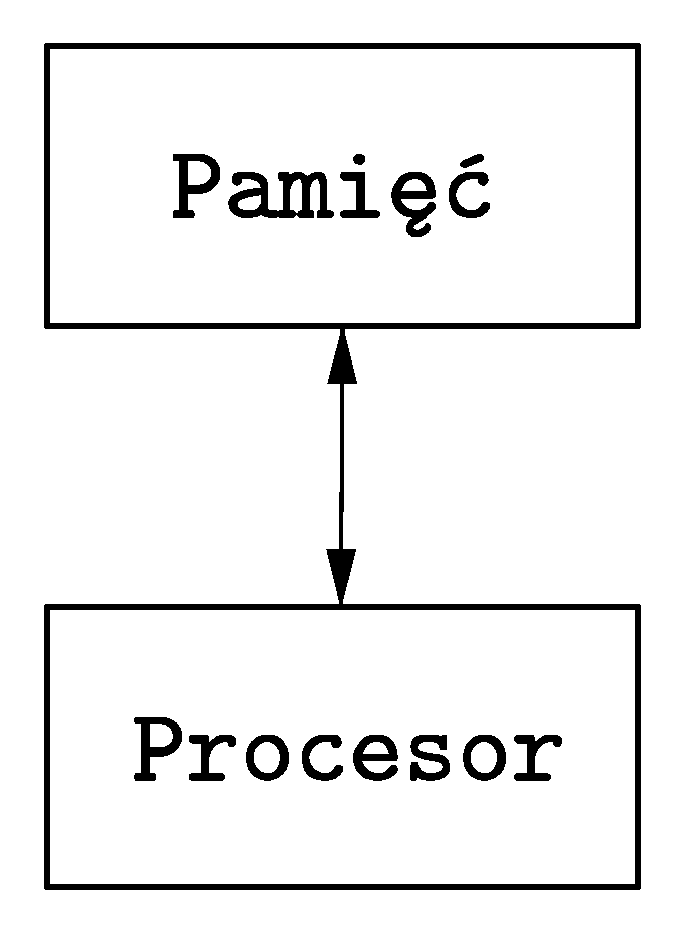
\includegraphics[width=7em]{images/Rys_RAM.eps}
% \caption{Model obliczeń sekwencyjnych RAM}
% \label{fig:ram}
% 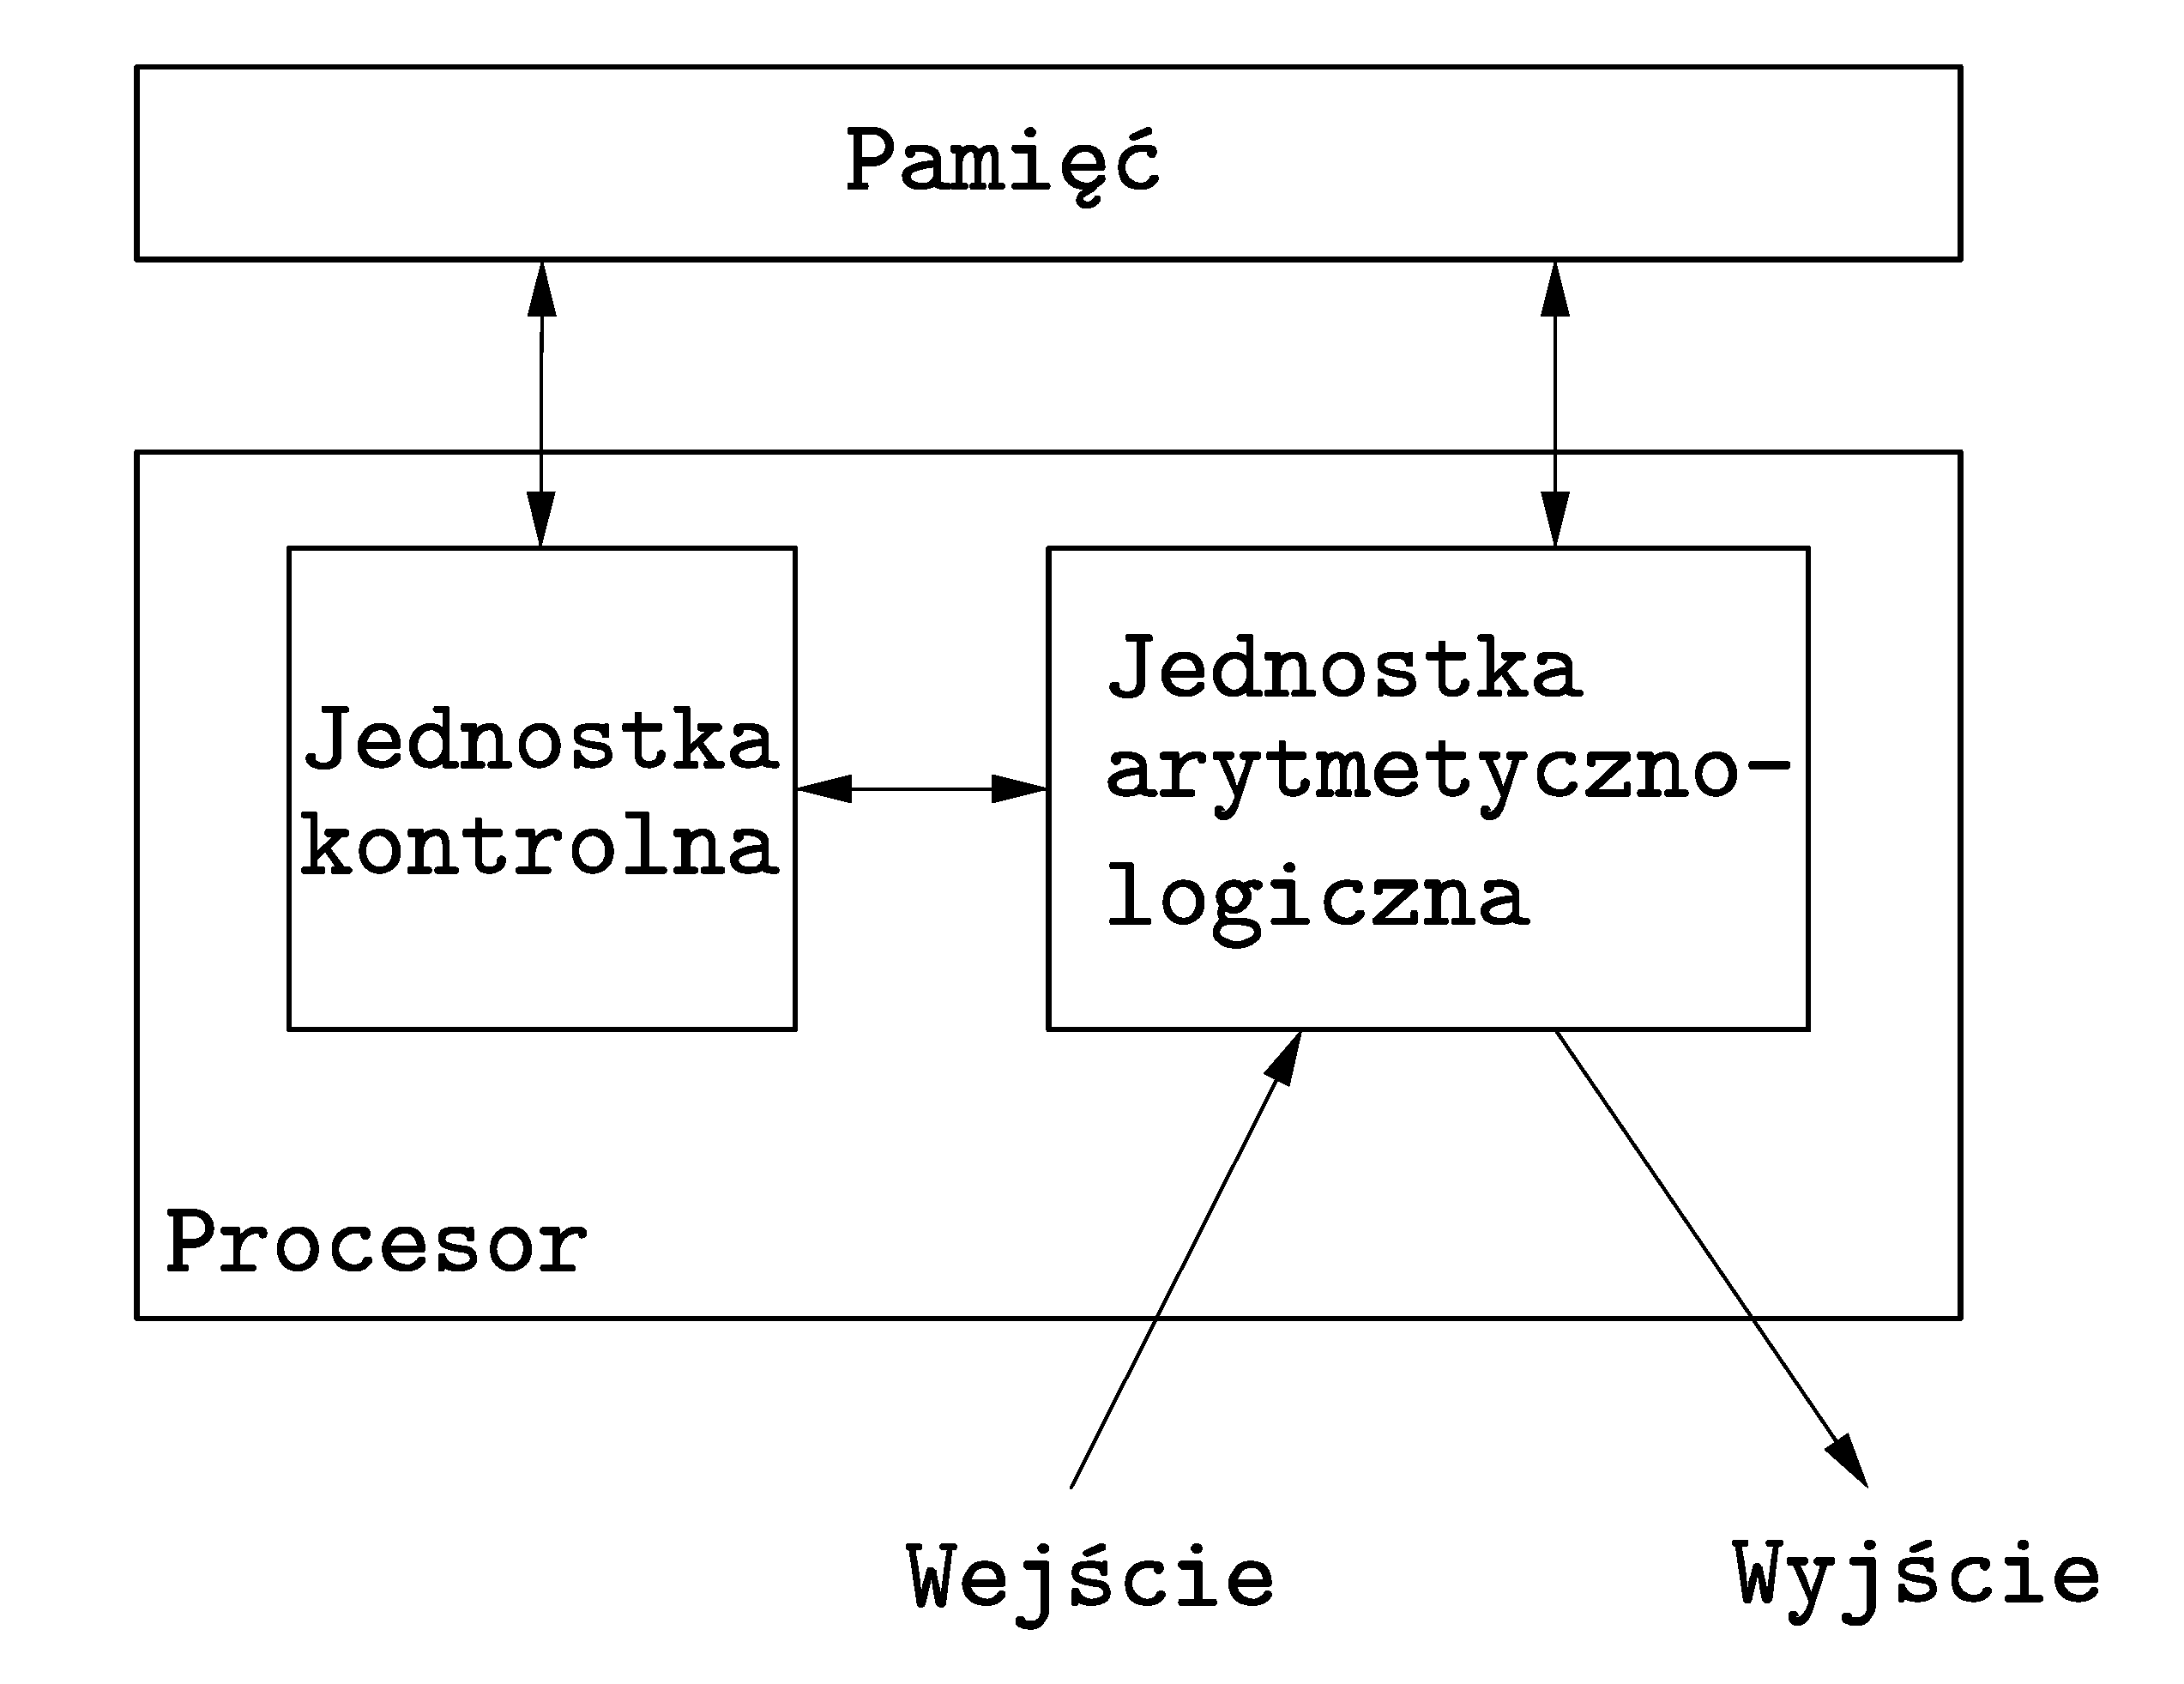
\includegraphics[width=7cm]{images/Rys_Neumann.eps}
% \end{figure}

\begin{table}[H]
\begin{center}
\caption{Przykładowa lista instrukcji procesora\cite{Czech}}
\label{tab:ram_instructions}
\begin{tabular}{|l|c|l|}
\hline
Instrukcja & Argument & Znaczenie \\ \hline
\texttt{LOAD} & \(k, a\) & \(R_k:=w(a)\) \\
\texttt{STORE} & \(k, b\) & \(M_{w(b)}:=R_{k}\) \\
\texttt{ADD} & \(k, c\) & \(R_{k}:=R_{k}+w(c)\) \\
\texttt{SUB} & \(k, c\) & \(R_{k}:=R_{k}-w(c)\)\\
\texttt{MULT} & \(k, c\) & \(R_{k}:=R_{k} \times w(c)\)\\
\texttt{DIV} & \(k, c\) & \(R_{k}:=\lfloor R_{k}/w(c)\rfloor\) \\
\texttt{JUMP} &  \(i\) & \(L:=i\) \\
\texttt{JPOS} & \(k,i\) & \texttt{if} \(R_k>0\) \texttt{then} \(L:=i\) \texttt{else} \(L:=L+1\) \\
\texttt{JZERO} & \(k,i\) & \texttt{if} \(R_k==0\) \texttt{then} \(L:=i\) \texttt{else} \(L:=L+1\) \\
\texttt{JNEG} & \(k,i\) & \texttt{if} \(R_k<0\) \texttt{then} \(L:=i\) \texttt{else} \(L:=L+1\) \\
\texttt{READ} & k & Wczytaj daną z urządzenia zewnętrznego do rejestru \(R_k\) \\
\texttt{WRITE} & k & Wydrukuj daną z rejestru \(R_k\) \\
\texttt{HALT} & & Zakończ obliczenie \\ \hline
\end{tabular}
\end{center}
\end{table}



\label{subsec:PRAM}
\subsection{Model PRAM}
Model wspólnej pamięci składa się z pewnej liczby procesorów, z których każdy posiada własną pamięć i może lokalnie wykonywać programy. Wszystkie procesory mogą komunikować się za pomocą wspólnej globalnej pamięci (rys. \ref{fig:model_shared}).

\begin{definicja}[Złożoność komunikacyjna\cite{Czech}]\label{def:communication_complexity}
Maksymalny rozmiar danych przesłanych w trakcie wykonywania algorytmu PRAM między pamięcią wspólną, a pamięcią lokalną dowolnego procesora nazywamy \emph{złożonością komunikacyjną}.
\end{definicja}

Każdemu procesorowi przypożądkowana jest niepowtarzająca się liczba naturalna. Jest to lokalnie dostępny indeks, numer procesora lub jego identyfikator.

\begin{figure}[h]
\centering
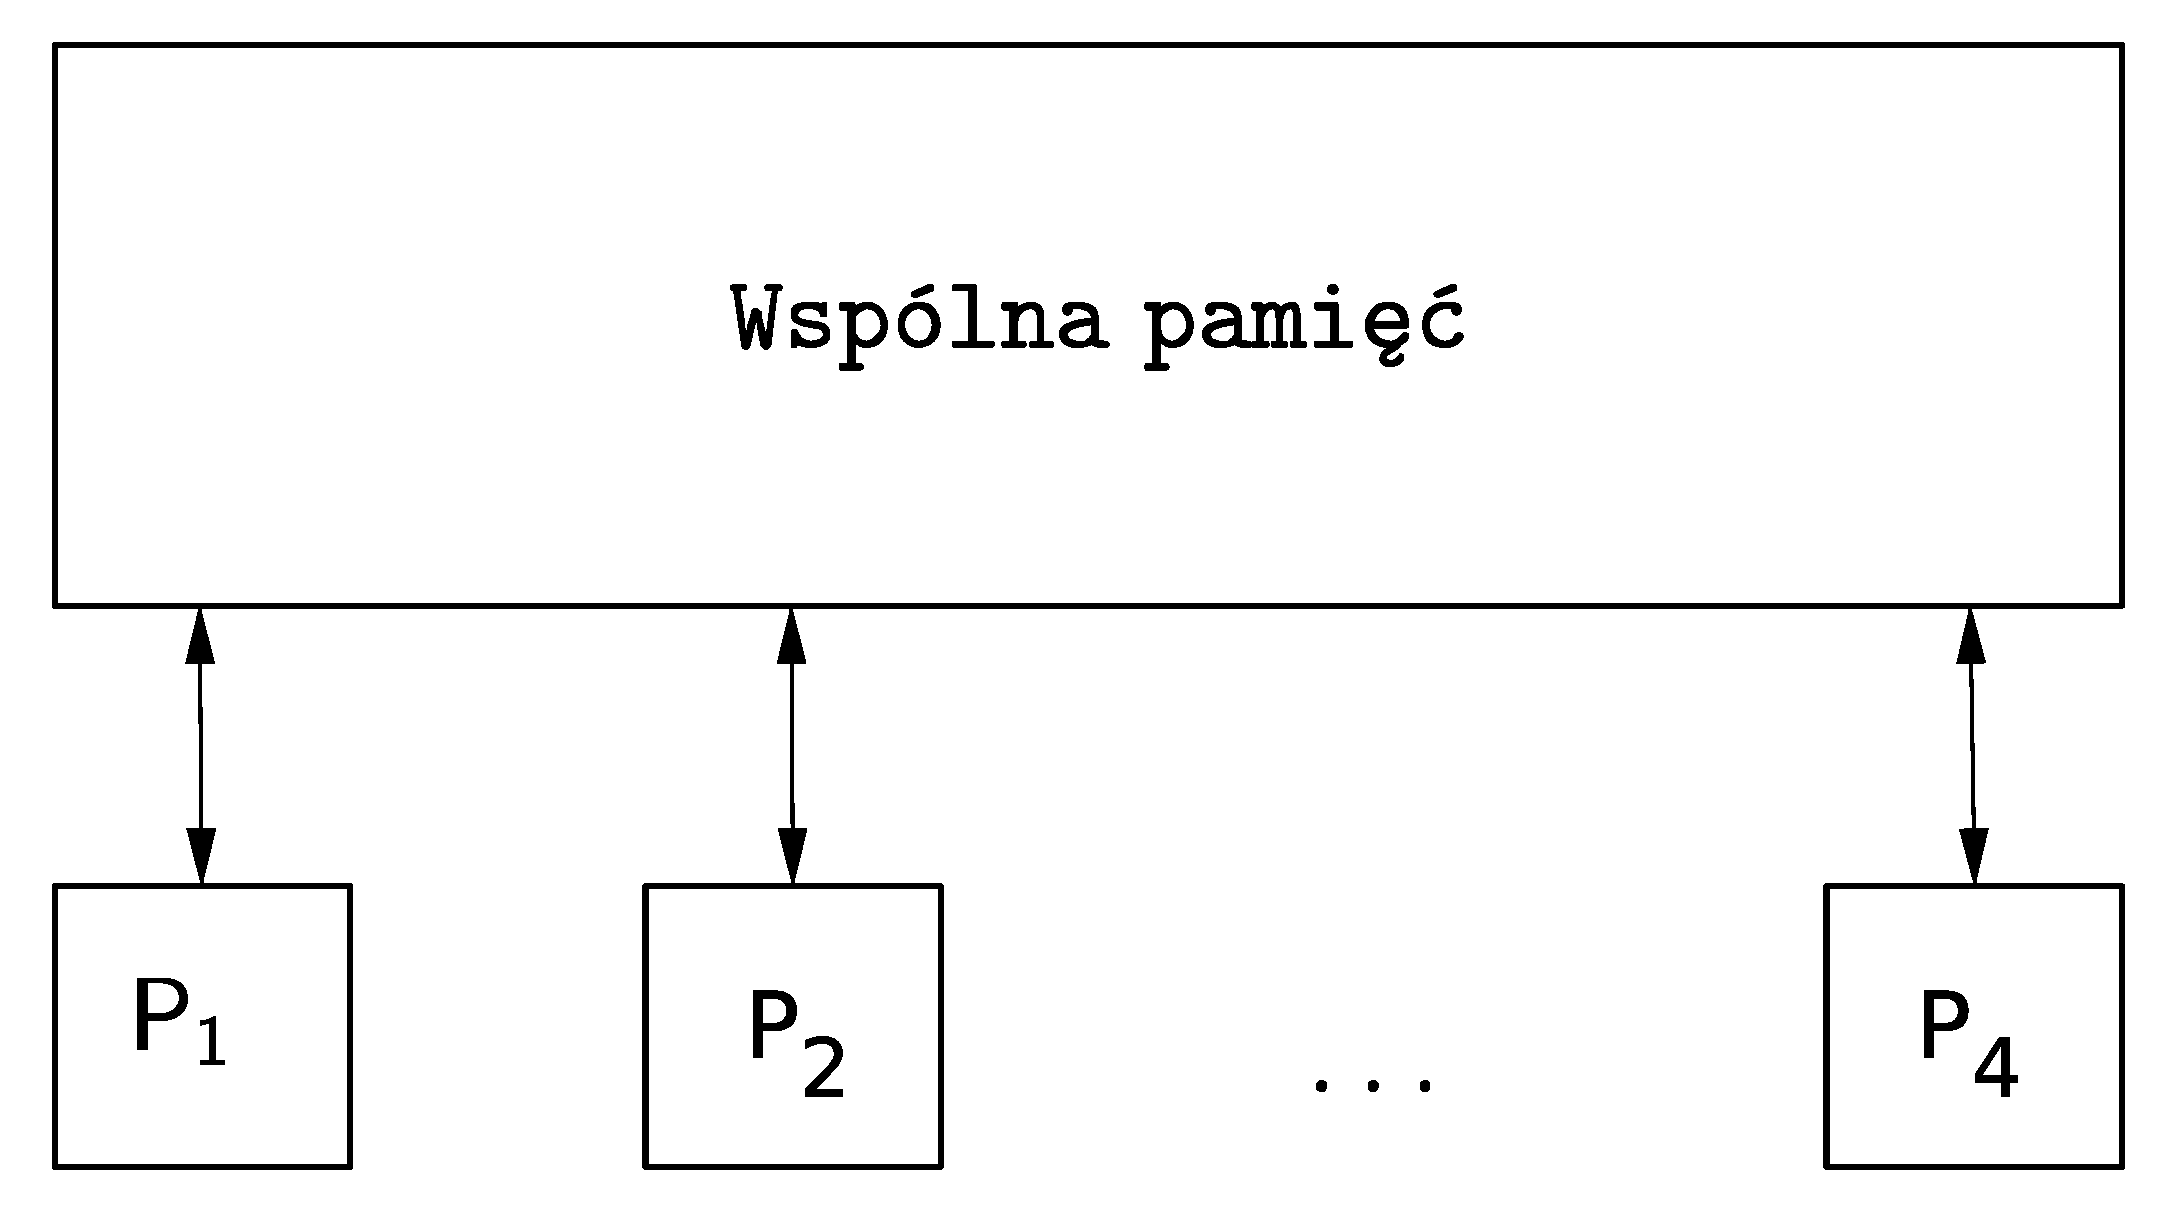
\includegraphics[width=20em]{images/Rys4.eps}
\caption{Model wspólnej pamięci}
\label{fig:model_shared}
\end{figure}


W modelu wspólnej pamięci wyróżniamy dwa podstawowe tryby operacji.
\begin{itemize}
\item Tryb synchroniczny. Wszystkie procesory działają synchronicznie według wspólnego zegara. Model ten nazywamy równoległą maszyną o dostepie swobodnym (PRAM, parallel random-access machine).


\item Tryb asynchroniczny. Każdy procesor pracuje według osobnego zegara. W tym trybie programista jest odpowiedzialny za odpowiednią synchronizację procesorów, jeśli zachodzi taka potrzeba. Dokładniej mówiąc, jeśli procesor ma pobrać dane, to odpowiedzialnością programisty jest upewnienie się, że odpowiednie dane są już uzyskane, ponieważ wartości wspólnych zmiennych są określane dynamicznie w trakcie wykonania programu na różnych procesorach.
\end{itemize}

Ponieważ każdy procesor może uruchomić swój program lokalnie, ten model jest typu MIMD w klasyfikacji Flynna. Znaczy to tyle, że każdy procesor może wykonać pewną instrukcję lub operację na danych niezależnie od tych wykonanych na jakimkolwiek innym procesorze w trakcie danej jednostki czasu.


% Dla danego algorytmu, rozmiar danych wymienionych pomiędzy pamięcią globalną i pamięcią lokalną różnych procesorów wyraża rozmiar \textbf{komunikacji} wymaganej przez algorytm.


Możemy wyróżnić kilka wariantów modelu PRAM w zależności od wymagań jakie postawimy odnośnie jednoczesnego dostępu kilku procesorów do tego samego adresu w pamięci globalnej.\\
\begin{itemize}
\item\textbf{EREW} -- algorytmy z wyłącznym odczytem i wyłącznym zapisem; nie pozwala na jednoczesny zapis do pamieci.
\item\textbf{CREW} -- algorytmy z jednoczesnym odczytem i wyłącznym zapisem; pozwala na jednoczesny  dostęp do pamięci dla instrukcji odczytu.
\item\textbf{CRCW} -- algorytmy z jednoczesnym odczytem i jednoczesnym zapisem.
\item\textbf{ERCW} -- algorytmy z wyłącznym odczytem i jednoczesnym zapisem.
\end{itemize}


Jeśli nie poczyni się żadnych dodatkowych założeń, to nie jest jasno określone, co zostanie zapisane w komórce pamięci w wyniku jednoczesnego zapisywania do niej przez wiele procesorów w algorytmie typu CRCW. W literaturze można spotkać wiele typów maszyny PRAM, które różnią się sposobami rozwiązywania konfliktów zapisu. Można wśród nich wyróżnić\cite{Cormen94}:
\begin{enumerate}
\item jednolity (ang. \emph{common}) – procesory muszą zapisać do tej samej komórki pamięci jednolitą wartość.
\item dowolny (ang. \emph{arbitrary}) – zapamiętywana jest dowolna wartość z wartości zapisywanych do tej samej komórki pamięci.
\item priorytetowy (ang. \emph{priority}) – zapamiętywana jest wartość zapisywana przez procesor o najmniejszym numerze.
\item mieszany (ang. \emph{combining}) – zapamiętywana wartość jest pewną, jednak ściśle określoną kombinacją zapisywanych wartości.
\end{enumerate}



\subsection{Model sieciowy}
Sposób łączenia układu procesorów w sieć nazywamy topologią sieci. Topologię sieci modelowować jako graf \(G=(N,E)\), gdzie każdy węzeł \(i\in N\) oznacza procesor, a każda krawędź \((i, j) \in E\) – dwukierunkową komunikację między procesorami \(i\) i \(j\). Przyjmujemy, że każdy procesor ma swoją lokalną pamięć i nie ma żadnej pamięci współdzielonej przez procesory (rys. \ref{fig:model_net}). Tak jak w przypadku modelu z pamięcią wspólną, operacje w sieci mogą być synchroniczne lub asynchroniczne.\\

\begin{figure}[b]
\centering
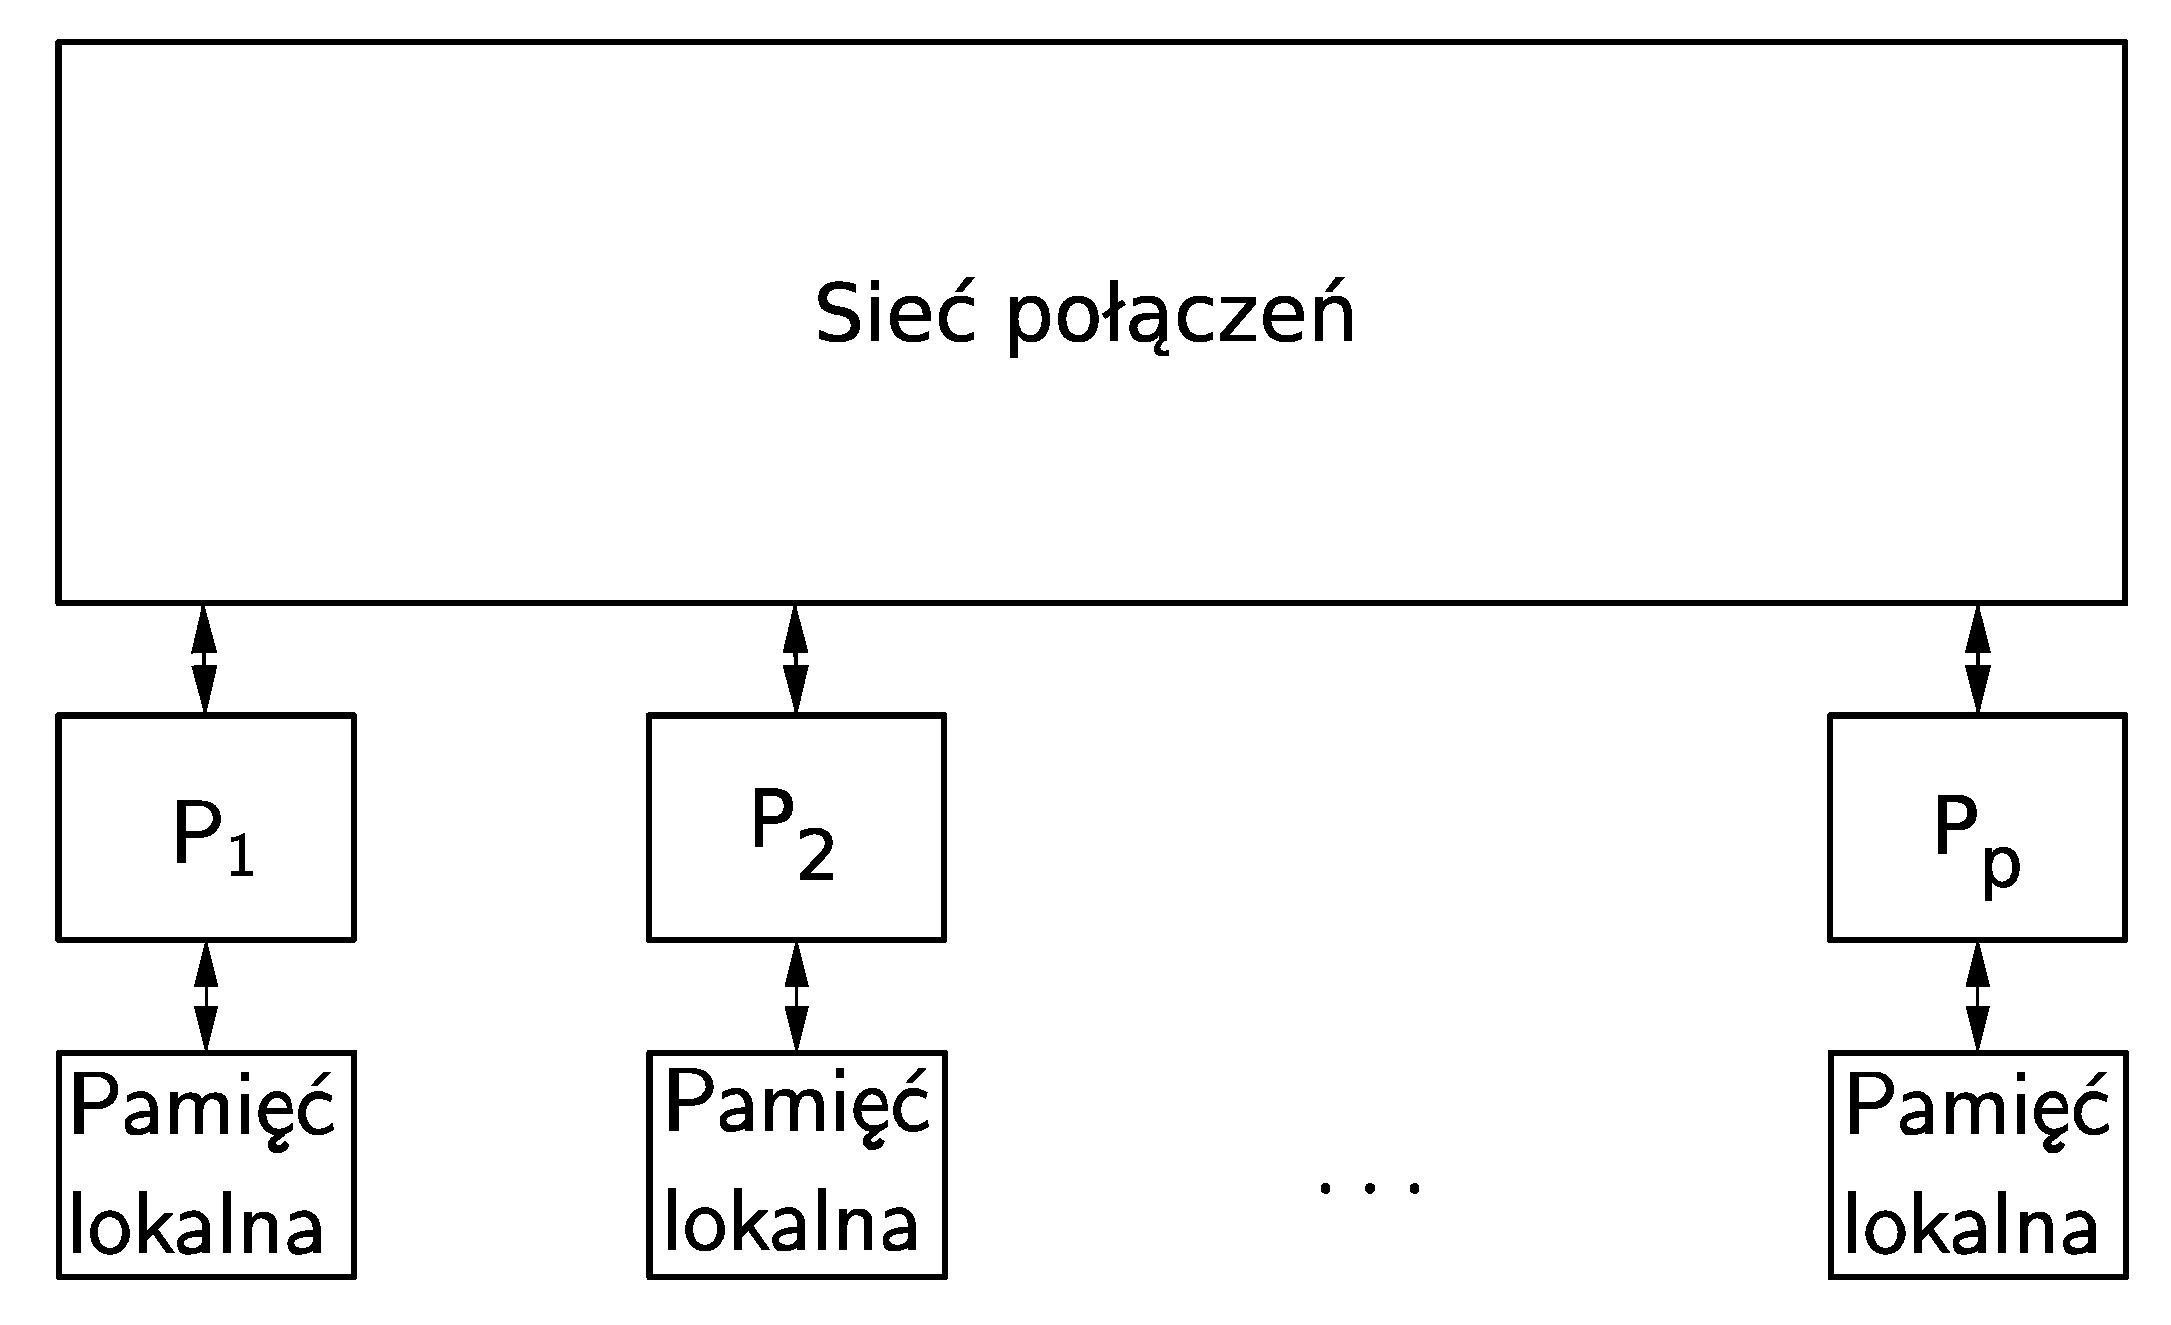
\includegraphics[width=22em]{images/Rys_net.eps}
\caption{Model wspólnej pamięci}
\label{fig:model_net}
\end{figure}

W opisie algorytmów dla modelu sieciowego potrzebujemy zdefiniować dwie instrukcje do opisania komunikacji między procesorami.
\begin{enumerate}
 \item send\((X,i)\)
 \item receive\((X,j)\)
\end{enumerate}

Procesor \(P\) wykonujący instrukcję \textbf{send} wysyła kopię \(X\) do procesora \(P_i\), następnie natychmiast przechodzi do wykonywania kolejnej instrukcji.\\
Procesor \(P\) wykonujący instrukcję \textbf{receive} zatrzymuje wykonanie programu aż do chwili, gdy otrzyma dane z procesora \(P_j\), a następnie przechowuje dane w \(Y\) i kontynuuje wykonanie programu.\\


Procesory pracujące w sieci asynchronicznej zarządzają swoimi zadaniami przez wymianę komunikatów. Schemat taki nazywamy modelem wymiany komunikatów. Procesory te niekoniecznie muszą być ze sobą sąsiadujące. 

%\begin{definicja}[Routing]
%Proces dostarczania każdego komunikatu od źródła do przeznaczenia nazywmy routingiem.
%\end{definicja}

Charakterysuje ją kilka parametrów:

\begin{enumerate}
 \item średnica – maksymalna odległość (krawędziowa) między dowolną parą węzłów; im miejsza, tym lepiej.
 \item maksymalny stopień wierzchołka – maksymalna liczba łączy do dane procesora
 \item szerokość połowienia sieci – minimalna liczba krawędzi, które muszą zostać usunięty, aby podzielić ją na dwie równe podsieci
 \item spójność krawędziowa – minimalna liczba krawędzi, które muszą ulec awarii, aby sieć stała się niespójna
 \item koszt sieci – koszt wykonania, zarządzania i utrzymania połączeń między procesorami; w najprostrzym przypadku mierzony liczbą krawędzi
\end{enumerate}



\begin{przyklad}[Sieć liniowa]
Model składa się z \(p\) procesorów \(P_1, P_2, \dots, P_p\) połączonych ze sobą w ciąg, tzn. procesor \(P_i\) połączony jest z procesorem \(P_{i-1}\) i \(P_{i+1}\), o ile takie istnieją. Średnica takiej sieci wynosi \(p-1\), jej maksymalny stopień wynosi \(2\).\\
\end{przyklad}

\begin{przyklad}[Torus]
Siecią w topologii torusa nazywamy sieć liniowa z połączonymi końcami.
\end{przyklad}

\begin{przyklad}{Sieć dwuwymiarowa}
Dwuwymiarowa sieć jest dwuwymiarową wersją sieci liniowej. Składa się ona z \(p=m^2\) procesorów ułożonych w siatkę \(m\times m\) taką, że procesor \(P_{i,j}\) jest połączony z procesorem \(P_{i\pm 1, j}\) i \(P_{i, j\pm 1}\).\\
Średnica takiej sieci złożonej z \(p=m^2\) procesorów wynos \(\sqrt{p}\) a jej maksymalny stopień \(4\)
\end{przyklad}

\begin{definicja}{Kostka Boola}\\
Niech \(i_{d-1}i_{d-2}\dots i_{0}\), gdzie \(0\leq i \leq p-1\) będzie binarną reprezentacją \(i\). Wówczas procesor \({i}\) jest połaczony z procesorem \(P_{i^(j)}\), gdzie \(i^{(j)}=i_{d-1}\dots \overline{i_j} \dots i_0\) i \(\overline{i_j} = 1 - i_j\). Innymi słowy, dwa procesory są ze sobą połączone wtedy i tylko wtedy, gdy ich wskaźniki różnią się tylko jednym bitem.\\
\end{definicja}

\begin{przyklad}{Sieć hipersześcienna}
Sieć w topologii hipersześcianu skłąda się z \(p=2^d\) procesorów połączonych w d-wymiarową kostkę Boola.\\

Hipersześcian ma strukurę rekursywną. Kostkę \(d\)-wymiarową możemy rozszerzyć do \(d+1\) wymiarów przez połączenie poszczególnych procesorów do \(d\)-wymiarowych kostek.\\

Średnica d-wymiarowego hipersześcianu wynosi \(d=\log{p}\). Jest tak ponieważ odległośc w grafie między dwoma procesorami \(P_i\) i \(P_j\) jest równa liczbie pozycji bitów, którymi wskaźniki \(i\) i \(j\) różnią się między sobą. Stąd jest ona mniejsza lub równa \(d\), a ponadto odległość między \(P_0\) a \(P_{2^d-1}\) wynosi d. Każdy węzeł jest stopnia \(d=\log{p}\).
\end{przyklad}	
\begin{figure}[h]
\centering
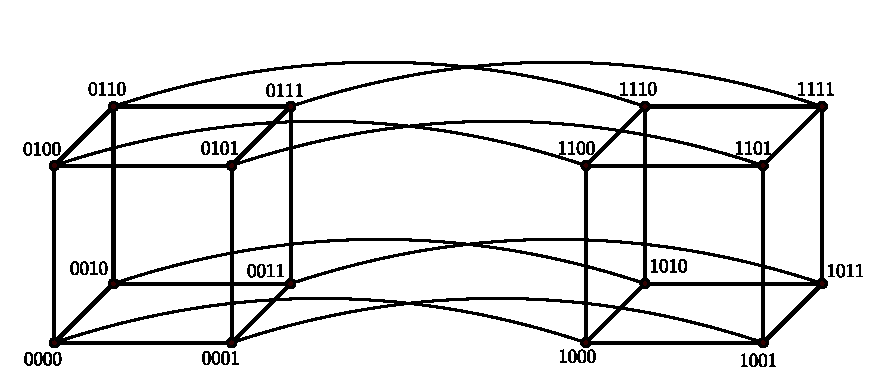
\includegraphics[width=32em]{images/systolic.eps}
\caption{Sieć w topologii hipersześcianu}
\label{fig:systolic}
\end{figure}




\section{Wybrane typy danych dla obliczeń rozproszonych}\label{sub:datatypes}
Powiedzmy, że wektor \(x\in\mathbb{R}^n\) jest rozdystrybuowany między pamięci lokalne sieci składającej się z \(p\) węzłów. Załóżmy wstępnie, że \(n=rp\). Do reprezentacji wektora \(x\) rozdystrybuowanego w sieci stosuje się najczęściej dwa następujące podejścia: zapis kolumnowy (ang. \emph{store-by-column}) oraz zapis wierszowy (ang. \emph{store-by-row}).

\noindent W pierwszym z nich\footnote{Używamy tutaj notacji programu Matlab; więcej informacji można znaleźć w \cite{Matlab}}, zapisie kolumnowym, rozpatrujemy wektor \(x\) jako macierz \(r\times p\):
\begin{align*}
x_{r\times p} = \left[x(1:r)\quad x(r+1:2r) \dots x(1+(p-1)r:n)\right],
\end{align*}
\noindent Każda \emph{kolumna} zapisana jest w osobnym węźle, tj. \( x (1+(\mu-1)r\colon \mu r) \in P_{\mu}\). (W tym kontekście predykat ,,\(x\in y\)'' oznacza ,,\(x\) jest zapisany w \(y\).'') Zauważmy, że każdy węzeł zawiera \emph{ciągłą} część wektora \(x\).


W zapisie wierszowym \(x\) traktujemy jako macierz wymiaru \(p\times r\):
\begin{align*}
x_{p\times r} = \left[x(1:p)\quad x(p+1:2p) \dots x((r-1)p:n)\right],
\end{align*}

Każdy \emph{wiersz} jest wówczas zapisany w odpowiednim węźle, tj. \(x (\mu \colon p \colon n)\in P_{\mu}\). Podejście to przypomina \emph{rozdawanie} (ang. \emph{wrap method}) danych węzłom sieci przez analogię do rozdawania kart graczom przy stole.

Jeśli \(n\) nie jest wielokrotnością \(p\) wówczas powyższe podejścia stosuje się z niewielką modyfikacją. Rozważmy zapis kolumnowy dla \(n=14\) i \(p=4\):
\begin{equation}
x^r=[\underbrace{x_1 x_2 x_3 x_4}_{P_0} | \underbrace{x_5 x_6 x_7 x_8}_{P_1} | \underbrace{x_9 x_{10} x_{11}}_{P_2} | \underbrace{x_{12} x_{13} x_{14}}_{P_3}]
\end{equation} 

Ogólniej, jeśli \(n = pr + q\), gdzie \(0\leq q < p-1\), to \(P_0, P_1, \dots, P_q\) mogą zgromadzić po \(r+1\) elementów, zaś \(P_{q+1}, P_{q+2}, \dots, P_{p-1}\) --- \(r\) elementów. Metoda wierszowa pozwala zgromadzić węzłowi \(P_{\mu}\) wektor \(x(\mu\colon p \colon n)\).

W podobny sposób możemy podejść do dystrybucji macierzy. Jeśli \(A\in\mathbb{R^{n\times n}}\) i \(n = rp\) możemy wyróżnić cztery podejścia:

\begin{table}[H]
\centering
\caption{Sposoby reprezentacji macierzy w sieci z \(q\) węzłami}
\begin{tabular}{ l | l | l }\label{tab:network_datatype}
  Orientacja & Styl & Zawartość węzła \\
  \hline
  Kolumnowy & Ciągły & \(A(\colon,\: 1+(\mu-1)r\colon \mu r)\) \\
  % \hline
  Kolumnowy & Rozdawany & \(A(\colon,\: \mu\colon p\colon n)\) \\
 % \hline
  Wierszowy & Ciągły & \(A(1+(\mu -1) r\colon\mu r,\: \colon)\) \\
  % \hline
  Wierszowy & Rozdawany & \(A(\mu \colon p\colon n,\: \colon)\) \\
  % \hline
 \end{tabular} 
 \end{table}

Metody dla macierzy blokowych są analogiczne do tych z tabeli \ref{tab:network_datatype}.

% \chapter{Wybrane algorytmy}

